%-------------------------------------------------------------------------------
% yum_bottom_panel
%-------------------------------------------------------------------------------
%
% \file        yum_bottom_panel.tex
% \library     Documents
% \author      Chris Ahlstrom
% \date        2015-06-06
% \update      2016-02-25
% \version     $Revision$
% \license     $XPC_GPL_LICENSE$
%
%     Provides the bottom_panel section of yoshimi-user-manual.tex.
%
%-------------------------------------------------------------------------------

\section{Bottom Panel}
\label{sec:bottom_panel}

\subsection{Bottom Panel Controls}
\label{subsec:bottom_panel_controls}

   The \textsl{Yoshimi} bottom panel provides quick access to some major
   features of the application.
   The bottom panel is shown in
   \figureref{fig:yoshimi_main_screen}.
%  figure~\ref{fig:yoshimi_main_screen} on
%  page~\pageref{fig:yoshimi_main_screen}.

   Here are the major elements of the bottom panel.

   \begin{enumber}
      \item \textbf{Part}
      \item \textbf{of}
      \item \textbf{Instrument Name}
      \item \textbf{Edit} (Instrument Edit Button)
      \item \textbf{Midi}
      \item \textbf{Mode}
      \item \textbf{Enabled}
      \item \textbf{Portamento}
      \item \textbf{Velocity Sens}
      \item \textbf{Velocity Offset}
      \item \textbf{Pan}
      \item \textbf{Pan Reset Button}
      \item \textbf{Volume}
      \item \textbf{Controllers}
      \item \textbf{Minimum Note}
      \item \textbf{Maximum Note}
      \item \textbf{m}
      \item \textbf{R}
      \item \textbf{M}
      \item \textbf{Key Shift}
      \item \textbf{Key Limit}
      \item \textbf{System Effect Sends 1}
      \item \textbf{System Effect Sends 2}
      \item \textbf{System Effect Sends 3}
      \item \textbf{System Effect Sends 4}
      \item \textbf{Sound Meter}
   \end{enumber}

   \setcounter{ItemCounter}{0}      % Reset the ItemCounter for this list.

   \itempar{Part}{bottom panel!part number}
   Part Number.

   Values: \texttt{1 to 16; 1 to 32; 1 to 64 }

   Show and set current part.  The maximum number of values depends on the
   \textbf{Part of} selection.

   \itempar{of}{bottom panel!part maximum}
   Maximum Number of Parts.

   Values: \texttt{16*, 32, 64}

   \textsl{Yoshimi} now has up to 64 parts in blocks of 16. One can now decide
   how many one wants to have available using this user-interface item.  By
   default these are wraped around the normal MIDI channels, so that parts 1,
   17, 33, and 49 all respond to channel 1 messages. This was originally
   implemented for Vector Control, working with up to four sounds on a channel
   (similar to the Yamaha SY hardware series).

   However, these additional parts have other less obvious uses. One of these
   is getting far more than 16 completely independent tracks addressed by just
   the 16 channels. Most tunes run with instruments having a relatively narrow
   pitch range, and this is what we can make use of.

   As an example, in \textsl{Yoshimi}'s main window select 64 parts, then on
   part 1 set (say) Steel Bass and maximum note as 52 (E).  Next select part 17
   and enable it (easiest to use the mixer panel for this) set Tunnel Piano,
   the *minimum* note as 53 and maximum as 71 (B).  Finally, enable part 33,
   set Rushes, and set it's minimum note as 72, but key shift down an octave.
   With a 61 note keyboard that gives one quite a useful working range, on just
   one channel.

   However, the idea really comes into its own with a sequencer like Rosegarden
   where one can record multiple parts over the full MIDI range and track them
   to the same channel. Also, in Rosegarden the parts can be separately named,
   and identified as Bass and Treble in the notation editor. This makes it very
   convenient for those wanting a more formal musical layout.

   So, with very little effort, one can now have 48 tracks playing at once!
   Ummm, one does need a decent processor though :)

   Yes, one could run more instances of Yoshimi on different MIDI ports, but
where's the fun in that?



   By default, all the upper parts (numbers greater than 16)
   are mapped to the same MIDI channel
   numbers as the lowest ones, but have independent voice and parameter
   settings. They cannot normally receive independent note or control
   messages. However, vector control will intelligently work with however
   many one has set, as will all the NRPN direct part controls.
   See \sectionref{subsection:vector_control}.

   This item is a fairly new feature of \textsl{Yoshimi} (as of version
   1.3.5).
   
   \itempar{Instrument Name}{bottom panel!instrument name}
   Instrument Name.
   Left-click to open the Bank window.
   Right-click to change the name of the current instrument.
   If one changes the name of the instrument, be sure to select
   \textbf{Menu / Instrument / Save Instrument} to preserve that change.

   The name now has color-coding to indicate the instrument's use of
   ADDsynth, SUBsynth, or PADsynth.  One can see the "red" color for ADDsynth
   in the figure for the bottom panel.  "Blue" would indicate SUBsynth, and
   "green" would indicate PADsynth.

   \itempar{Edit}{bottom panel!instrument edit}
   Instrument Edit button.
   This button brings up the instrument-edit dialog shown in
   \figureref{fig:instrument_edit_dialog}.

   This dialog provides a very broad overview of the instrument, and
   provides access to far more detailed dialogs to edit the instrument.
   This dialog is explained in detail in
   \sectionref{subsec:bottom_panel_instrument_edit}.

   \itempar{Midi}{bottom panel!MIDI channel}
   MIDI Channel.

   Values: \texttt{1 to 16}

   \itempar{Mode}{bottom panel!mode}
   Mode. Poly.
   Sets the mode (polyphonic/monophonic/legato).
   In polyphonic mode, multiple simultaneous notes are supported.
   (How many at maximum?).
   In monophonic mode, only one note is supported.
   In legato mode, the sound flows smoothly from note to note without
   any breaks.

   Values: \texttt{Poly, Mono, Legato}

   \itempar{Enabled}{bottom panel!instrument enable}
   Enable the part. If the Part is disabled it doesn't use CPU time.

   Values: \texttt{Off*, On}

   \itempar{Portamento}{bottom panel!portamento enable}
   Enable/disable the portamento.
   One can set the duration and other parameters by opening the Controllers
   window.

   Values: \texttt{Off*, On}

   \itempar{Velocity Sens}{bottom panel!velocity sensing}
   Velocity Sensing Function.

   Values: \texttt{0 to 127, 64*}

   \itempar{Velocity Offset}{bottom panel!velocity offset}
   Velocity Offset.

   Values: \texttt{0 to 127, 64*}

   \itempar{Pan}{bottom panel!pan}
   Pan.

   Values: \texttt{0 to 127, 64*}

   \itempar{Pan (reset)}{bottom panel!pan reset}
   Reset Pan to Middle (64).

   \itempar{Volume}{bottom panel!volume}
   Instrument Volume.

   Values: \texttt{0 to 127, 96*}
 
   The default volume for ADD parts (overall) and SUB parts is 96; the
   default volume for SUB parts is 90; the ADD voice volumen is 100; and
   effects volumes vary heavily with the effect.

   \itempar{Minimum Note}{bottom panel!minimum note}
   Minimum note the part receives.

   Values: \texttt{0* to 127}

   \itempar{Maximum Note}{bottom panel!maximum note}
   Maximum note the part receives.

   Values: \texttt{0 to 127*}

   \itempar{m}{bottom panel!m}
   Minimum Note Capture Button.

   Set minimum note to last note played.

   \itempar{R}{bottom panel!R}
   Minimum and Maximum Note Reset Button.

   Reset the minimum key to 0 and the maximum key to 127.

   \itempar{M}{bottom panel!M}
   Maximum Note Capture Button.

   Set maximum note to last pressed key.

   \itempar{Key Shift}{bottom panel!key shift}
   Key Shift.

   Values: \texttt{-12 to 12, 0*}

   \itempar{Key Limit}{bottom panel!key limit}
   Maximum keys for this part.

   Values: \texttt{0 to 55, 15*}

   \itempar{System Effect Sends 1, 2, 3, and 4}{bottom panel!system effect sends}

   TODO:  Describe how these sends work.
   \index{todo!SES123}

   Values: \texttt{0 to 127*}

   \itempar{Sound Meter}{bottom panel!sound meter}
   VU Meter.  Sound Meter.

   This discussion of "Audio Output and Levels"
   comes from \texttt{Output Levels.txt}.

   At the bottom of the main window there is a pair of horizontal grids
   representing a bargraph type display. The upper one is for the left hand
   channel and the lower one for the right hand one. The grid divisions each
   represent 1 dB, and the brighter divisions are therefore 5 dB. The thicker
   bright divisions therefore being 10 dB. The overall scale range is -48 dB to
   0 dB.

   As the output level rises pale blue strips will light up in these grids.
   These fast responding bars are the peak levels and should never be allowed
   to go above 0 dB, otherwise the output is likely to be clipped and distorted.
   There is also a pair of boxes on the end of these grids which will show the
   highest peak level seen. If clipping has happened the box background will
   change from black to red.

   To clear clip and peak level indication click on this area.

   As well as the peak level, the display shows a much slower responding RMS
   level, as a yellow line on top of the blue bar. This gives and indication of
   the apparent accoustic power.

   If one opens the panel window one will see vertical bargraphs for each
   individual part. On these, the faint bars are 5dB steps and the bright ones
   10dB. The peak leve isn't shown numerically, but if one exceeds 0dB a thick
   red line will appear at the top of the bargraph. This is also cleared from
   the box in the main window.

   (More information to come).

\paragraph{Tip: Using the VU Meter}
\label{paragraph:tips_using_the_vu_meter}
\index{tips!vu meter}

   The VU meter topic is very interesting, because one of the problems
   is a tendency to overdrive by way of sustain pedal.  At the last test it
   showed up in the output before it showed up in the VU meter, so
   the VU meter should help a lot in analysis.

   One way to avoid overdrive is to keep polyphony to 20 on each patch (two
   or three patches per \textsl{Yoshimi} instance, with two or three
   \textsl{Yoshimi} simultaneous instances depending on the patch).

   Another item which helps a lot is compression (for example, the Calf
   multiband compressor is amazingly good.

\subsection{Bottom Panel / Controllers}
\label{subsec:bottom_panel_controllers}

\begin{figure}[H]
   \centering 
   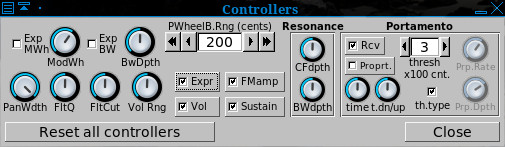
\includegraphics[scale=1.0]{bottom-panel/controllers-dialog.jpg}
   \caption{Controllers Dialog}
   \label{fig:controllers_dialog}
\end{figure}

   \begin{enumber}
      \item \textbf{Exp MWh}
      \item \textbf{ModWh}
      \item \textbf{Exp BW}
      \item \textbf{BwDepth}
      \item \textbf{PanWdth}
      \item \textbf{FltQ}
      \item \textbf{FitCut}
      \item \textbf{Vol Rng}
      \item \textbf{PWheelB.Rng}
      \item \textbf{Expr}
      \item \textbf{FMamp}
      \item \textbf{Vol}
      \item \textbf{Sustain}
      \item \textbf{Resonance} (section)
      \item \textbf{PortaMento} (section)
      \item \textbf{Reset all controllers}
      \item \textbf{Close}
   \end{enumber}

   \setcounter{ItemCounter}{0}      % Reset the ItemCounter for this list.

   \itempar{Exp MWh}{controllers!expression mod wheel}
   Exponential Modulation Wheel.
   Changes the modulation scale to exponential.

   Values: \texttt{Off*, On}

   \itempar{ModWh}{controllers!mod wheel depth}
   Modulation Wheel Depth.

   Values: \texttt{0 to 127, 80*}

   \itempar{Exp BW}{controllers!exp bandwidth controller}
   Exponential Bandwidth Controller.
   Changes the bandwidth scale to exponential.

   Values: \texttt{Off*, On}

   \itempar{BwDepth}{controllers!bandwidth depth}
   Bandwidth Depth.

   Values: \texttt{0 to 127, 64*}

   \itempar{Exp BW}{controllers!bandwidth depth}
   Exponental Bandwidth.
   Changes the bandwidth scale to exponential.

   Values: \texttt{0 to 127, 64*}

   \itempar{PanDpth}{controllers!panning depth}
   Panning Depth.

   Values: \texttt{0 to 64*}

   \itempar{FltQ}{controllers!filter Q depth}
   Filter Q (resonance) Depth.

   Values: \texttt{0 to 127, 64*}

   \itempar{FltCut}{controllers!filter cutoff depth}
   Filter Cutoff Frequency Depth.

   Values: \texttt{0 to 127, 64*}

   \itempar{Vol Rng}{controllers!volume range}
   Volume Range.

   Values: \texttt{64 to 127, 64*}

   \itempar{PWheelB.Rng}{controllers!pitch wheel range}
   Pitch Wheel Bend Range (cents).
   100 cents = 1 halftone.

   Values: \texttt{-6400 to 6400, 200*}

   \itempar{Expr}{controllers!expression}
   Expression Enable.
   Enable/disable expression.

   Values: \texttt{Off, On*}

   \itempar{FMamp}{controllers!fm amplitude}
   FM Amplitude Enable.
   Enable/disable receiving Modulation Amplitude controller (76).

   Values: \texttt{Off, On*}

   \itempar{Vol}{controllers!volume enable}
   Volume Enable.

   Values: \texttt{Off, On*}

   Enable/disable receiving volume controller.
   Sensitivity to MIDI volume change (CC7) is now variable in 'Controllers'
   in the same way as pan width etc. The nnumeric range is 64 to 127; the
   default at 96 gives the same sensitivity as before at -12dB relative to
   the GUI controls. 127 gives 0dB and 64 gives -26dB

   \itempar{Sustain}{controllers!sustain pedal enable}
   Sustain Pedal Enable.
   Enable/disable sustain pedal.

   Values: \texttt{Off, On*}

   \itempar{Reset all controllers}{controllers!reset all}
   Reset All Controllers.

   \itempar{Close}{controllers!close}
   Close Window.

\subsubsection{Bottom Panel / Controllers / Resonance}
\label{subsubsec:bottom_panel_controllers_resonance}

   \setcounter{ItemCounter}{0}      % Reset the ItemCounter for this list.

   \itempar{CFdepth}{controllers!resonance CF depth}
   Resonance Center Frequency Depth,
   Center Frequency Controller Depth.

   Values: \texttt{0 to 127, 64*}

   \itempar{BWdepth}{controllers!resonance BW depth}
   Resonance Bandwidth Depth,
   Resonance Bandwidth Controller Depth.

   Values: \texttt{0 to 127, 64*}

\subsubsection{Bottom Panel / Controllers / Portamento}
\label{subsubsec:bottom_panel_controllers_portamento}

   \setcounter{ItemCounter}{0}      % Reset the ItemCounter for this list.

   \itempar{Rcv}{controllers!portamento receive}
   Portamento Receive,
   Receive Portamento Controllers.
   Determines if the part receives Portamento On/Off (65) controller.

   Values: \texttt{Off, On*}

   \itempar{Proprt.}{controllers!portamento proportional}
   Portamento Proportional,
   Enable Proportional Portamento (over fixed portamento).

   Values: \texttt{Off*, On}

   \itempar{time}{controllers!portamento time}
   Portamento time.
   The duration of the portamento.

   Values: \texttt{0 to 127, 64*}

   \itempar{t.dn/up}{controllers!portamento time, down/up}
   Portamento Time Stretch (up/down).

   Values: \texttt{0 to 127, 64*}

   \itempar{threshx100 cnt.}{controllers!portamento threshold}
   Threshold of the Portamento.

   Values: \texttt{0 to 127, 3*}

   Minimum or maximum difference of notes in order
   to do the portamento (x 100 cents).
   It represents the minimum or the maximum number of halftones (or hundred
   cents) required to start the portamento. The difference is computed
   between the last note and current note.

   The threshold refers to the frequencies and not to MIDI notes (one should
   consider this if one uses microtonal scales).

   \itempar{th.type}{controllers!portamento threshold type}
   Threshold Type (min/max).
   Checked means that the portamento activates when the difference of
   frequencies is above the threshold ("thresh"); not checked is for below
   the threshold.

   Values: \texttt{Off, On*}

   \itempar{Propt.}{controllers!portamento proportional}
   Proportional Portamento.
   If set, the portamento is proportional to ratio of frequencies.

   Values: \texttt{Off, On*}

   \itempar{Prp.Rate}{controllers!portamento rate}
   Distance required to double change from nonproportional
   portamento time.
   The ratio needed to double the time of portamento.

   Values: \texttt{0 to 127, 80*}, requires \textbf{Proprt.} = \texttt{On}

   \itempar{Prp.Depth}{controllers!portamento depth}
   The difference from nonproportional portamento.

   Values: \texttt{0 to 127, 90*}, requires \textbf{Proprt.} = \texttt{On}

\subsection{Bottom Panel Instrument Edit}
\label{subsec:bottom_panel_instrument_edit}

   The main instrument-editing dialog is relatively simple, and provides for
   editing information that identifies the instrument, and buttons to access
   the more complex dialogs of the ADDsynth, SUBsynth, PADsynth, Kit Edit,
   and Effects components.

%  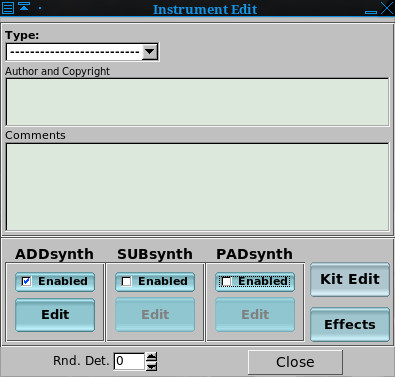
\includegraphics[scale=1.0]{bottom-panel/edit-instrument.jpg}

\begin{figure}[H]
   \centering 
   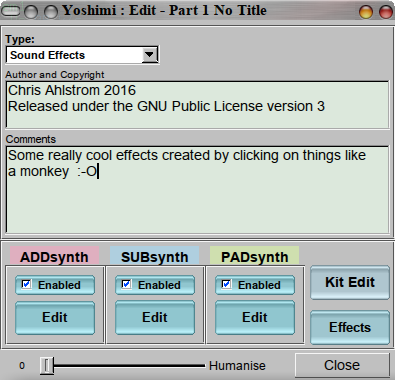
\includegraphics[scale=1.0]{1.3.5/edit-instrument.png}
   \caption{Instrument Edit Dialog}
   \label{fig:instrument_edit_dialog}
\end{figure}

   This dialog provides a very broad overview of the instrument, and
   provides access to far more detailed dialogs to edit the instrument.
   This dialog is called up by the \textbf{Edit} button on the bottom panel
   of the main \textsl{Yoshimi} main screen.

   \begin{enumber}
      \item \textbf{Type}
      \item \textbf{Author and Copyright}
      \item \textbf{Comments}
      \item \textbf{ADDsynth}
      \begin{enumber}
         \item \textbf{Enabled}
         \item \textbf{Edit}
      \end{enumber}
      \item \textbf{SUBsynth}
      \begin{enumber}
         \item \textbf{Enabled}
         \item \textbf{Edit}
      \end{enumber}
      \item \textbf{PADsynth}
      \begin{enumber}
         \item \textbf{Enabled}
         \item \textbf{Edit}
      \end{enumber}
      \item \textbf{Kit Edit}
      \item \textbf{Effects}
      \item \textbf{Rnd. Det.}
      \item \textbf{Close}
   \end{enumber}

   The ADDsynth, SUBsynth, PADsynth, Kit Edit, and Effects
   dialogs are detailed in separated sections, as they are all
   very complex dialogs with many sub-dialogs.

   \itempar{Type}{edit!category}
   Instrument Type.
   Instrument Category.

   This dropdown dialog allows one to tag the type of instrument, to
   indicate what category of instruments it fits into.
   The following figure shows the types.

\begin{figure}[H]
   \centering 
   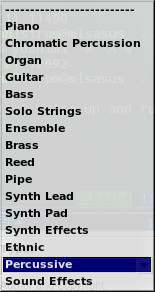
\includegraphics[scale=1.0]{bottom-panel/edit-instrument-type.jpg}
   \caption{Instrument Type Dropdown}
   \label{fig:instrument_type_dropdown}
\end{figure}

   Values: \texttt{Piano, Chromatic Percussion, Organ, Guitar, Bass,
              Solo Strings, Ensemble, Brass, Reed, Pipe,
              Synth Lead, Synth Pad, Synth Effects, Ethnic,
              Percussive, Sound Effects}

   \itempar{Author and Copyright}{edit!author/copyright}
   This field provides space for identifying the author, copyright, and
   license for the part.

   \itempar{Comments}{edit!comments}
   Allows free-form comments and notes to be entered.

   \itempar{ADDsynth}{edit!addsynth}

   \begin{enumber}
      \item \textbf{Enabled}.
      Enables this synth type to be used in the part/instrument.
      When enabled, its marker color, red, is shown.
      \item \textbf{Edit}.
      Brings up the editing dialog presented in
      \figureref{fig:addsynth_edit_dialog}.
      There one will find a full discussion of that dialog.
   \end{enumber}

   \itempar{SUBsynth}{edit!subsynth}

   \begin{enumber}
      \item \textbf{Enabled}.
      Enables this synth type to be used in the part/instrument.
      When enabled, its marker color, blue, is shown.
      \item \textbf{Edit}.
      Brings up the editing dialog presented in
      \figureref{fig:subsynth_edit_dialog}.
      There one will find a full discussion of that dialog.
   \end{enumber}

   \itempar{PADsynth}{edit!padsynth}

   \begin{enumber}
      \item \textbf{Enabled}.
      Enables this synth type to be used in the part/instrument.
      When enabled, its marker color, green, is shown.
      \item \textbf{Edit}.
      Brings up the editing dialog presented in
      \figureref{fig:padsynth_edit_dialog}.
      There one will find a full discussion of that dialog.
   \end{enumber}

   \itempar{Kit Edit}{edit!kit}
   Brings up the editing dialog presented in
   \figureref{fig:kit_edit_dialog}.
   There one will find a full discussion of that dialog.

   \itempar{Effects}{edit!effects}
   Brings up the editing dialog presented in
   \figureref{fig:effects_edit_none}
   There one will find a full discussion of that dialog.

   \itempar{Rnd. Det.}{edit!rnd det}
   Small Random Detune.

   Values: \texttt{0* to 20}

   This value is an experimental feature.  It would lend some complexity or
   piquancy to the part/instrument.

   \itempar{Close}{edit!close}
   Closes the Edit window.

%-------------------------------------------------------------------------------
% vim: ts=3 sw=3 et ft=tex
%-------------------------------------------------------------------------------
